\documentclass[12pt]{article}
\usepackage[italian]{babel}
\usepackage{graphicx}
\usepackage{titling}
\usepackage{multicol}
\usepackage{titlesec}
\usepackage{hyperref} %To setup table of content links
\usepackage{amssymb}
%\usepackage{changepage}
\usepackage{geometry} %To modify margins
\usepackage{gensymb}


 \geometry{
 a4paper,
 total={170mm,257mm},
 left=20mm,
 top=20mm,
 }

\hypersetup{
    colorlinks,
    citecolor=black,
    filecolor=black,
    linkcolor=black,
    urlcolor=black
}


%=========================================
\begin{document}


\begin{titlepage}
   \begin{center}
       \vspace*{1cm}
 
	\large
      {\huge \textbf{Elaborato ESI Stabilizzazione video} }
 
       \vspace{1.5cm}
 
       \textbf{Nicolò Fretti - Stefano Nicolis}\\
	\textbf{A.A. 2020-2021}\\
	\vspace{0.35cm}
	\textbf{\today}

\vfill
\begin{figure}[h!]
	\begin{center}
	  
\includegraphics[height=6cm, width=6cm]{media/logounivr}
	\end{center}
\end{figure}
 
	\vfill
 	\textbf{Corso di \\
       Elaborazioni dei Segnali e Immagini\\}
 
       \vspace{3cm}
 
      \begin{multicols}{2}
      \textbf{Università degli Studi di Verona\\
	 Dipartimento di Informatica}
	\end{multicols}
 
   \end{center}
\end{titlepage}


\tableofcontents

\clearpage

\section{Introduzione}
Viene richiesta la progettazione del codice MatLab per la stabilizzazione un video. Quest'ulti-
ma, preso in input un video, deve operare sulla traslazione e rotazione dello stesso in modo da
stabilizzarlo secondo un'ancora, ovvero una porzione di video selezionata dall'utente.
\textbf{Note}:
\begin{itemize}
\item È stato scelto di stabilizzare l'ancora al centro del frame, in maniera tale da notare meglio la stabilizzazione rispetto alla porzione di video selezionata
\item Gli spazi vuoti lasciati dall'imagine traslata vengono riempiti di nero
\item Viene assunto che il video sia stato registrato da una persona, e quindi tra un frame e l'altro non ci sono variaizioni di angolo maggiori di n$^{\circ}$, dove n, per questioni di efficienza, dipende dalla risoluzione del video
\end{itemize}

\clearpage
\section{Approccio utilizzato}
L'operazione che rende possible la stabilizzazione e la cross-corellazione. Intuitivamente, permette di scorrere un determinato template su un'immagine di riferimento e trovare la posizione in cui il template e più simile all'immagine.
L'algoritmo, presa in input l'ancora, esegue su ogni frame le seguenti operazioni:

\begin{itemize}
\item ricerca e applicazione dell'angolo di rotazione sul frame attuale
\item cross-correlazione tra ancora e frame ruotato per ricavare l'offset
\item traslazione del frame in base all'offset ricavato
\end{itemize}

\subsection{Ricerca angolo di rotazione}
Per la selezione dell'angolo migliore vengono eseguite due passate di ricerca sul frame, nella prima passata viene fatta una ricerca `grossolana', ovvero ricerchiamo l'angolo vericando il valore di cross correllazione entro un intervallo che diminuisce al crescere della risoluzione, dato l'intervallo viene eseguita una ricerca ogni 10$^{\circ}$.

\begin{figure}[h!]
	\begin{center}
	  \fbox{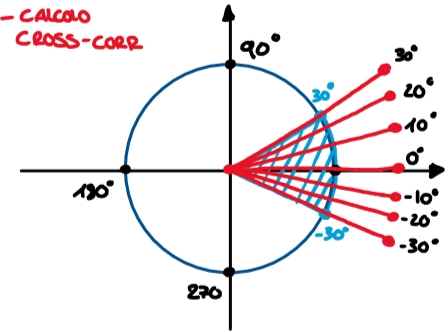
\includegraphics[scale=0.6]{media/chart_1}}
	  \caption{Esempio passata inziale con risoluzione < 640*480}
	\end{center}
\end{figure}

Mentre nella seconda passata viene cercato l'angolo in un intervallo piccolo con uno step
che dipende dalla risolzione del video.

\begin{figure}[h!]
	\begin{center}
	  \fbox{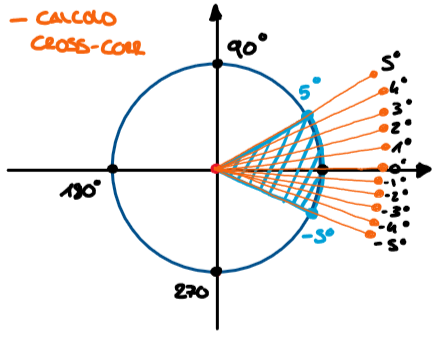
\includegraphics[scale=0.6]{media/chart_2}}
	  \caption{Esempio seconda passata con risoluzione < 640*480, con 0$^{\circ}$ come risulato della prima passata}
	\end{center}
\end{figure}

Trovato l'angolo, viene ruotato il frame in base ad esso. In seguito viene effettuata un'altra cross-correlaziona per trovare l'offset con cui eseguire la traslazione. Ripetendo queste operazioni per ogni frame il risultato e un video che presenta l'ancora al centro del frame, stabile rispetto a traslazione e rotazione.

\clearpage
\section{Utilizzo}
Il programma si presenta all'utente con una schermata molto semplice, composta da due
schermate inizialmente vuote, che mostrano il video originale e la versione stabilizzata.
In basso alla nestra vi sono tre tasti:
\begin{itemize}
	\item Scegli video: permette di cambiare il video da stabilizzare
	\item Stabilizza: scelta dell'ancora rispetto a cui stabilizzare
	\item Play: riproduci il video
\end{itemize}

\begin{figure}[h!]
	\begin{center}
	  \fbox{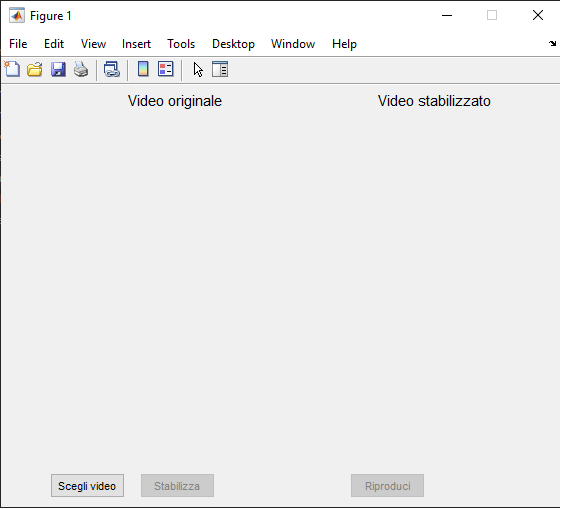
\includegraphics[scale=0.6]{media/UI}}
	  \caption{Schermata del programma}
	\end{center}
\end{figure}
\end{document}